\chapter{Wirtualizacja}

Jednym z zastosowań wirtualizacji jest jednoczesne uruchomienie wielu instancji systemu operacyjnego na tym samym sprzęcie fizycznym. Oprogramowanie wirtualizacyjne rozdziela zasoby procesora, pamięci oraz operacje wejścia-wyjścia, przydzielając je odseparowanym od siebie wirtualnym maszynom \cite{biblia_linux}.

Wirtualizacja rozwijana jest od lat 60. XX wieku. Na początku opracowywana była przez firmę IBM z myślą o wyspecjalizowanych mainframe'ach. W tamtym okresie technologia ta nie zyskała jednak popularności. Było to spowodowane głównie ograniczeniami technologicznymi i częściej wykorzystywanym \textit{time-sharingiem}, który pozwalał wielu użytkownikom wykonywać operacje na jednej maszynie w tym samym czasie \cite{idkrtm, arundel}. 

Przełom nastąpił wraz ze wzrostem roli infrastruktury informatycznej w biznesie. Jednym z największych ówczesnych problemów był transfer oprogramowania na nowy sprzęt. Było to zwykle niemożliwe bez wprowadzenia zmian w samym oprogramowaniu lub odtworzeniu go na architekturę nowej maszyny. To z kolei generowało koszty i wymagało czasu. 

Kolejną trudnością był sposób przechowywania aplikacji na serwerach. Jednoczesne uruchamianie wielu aplikacji na pojedynczym fizycznym serwerze nierzadko stwarzało problemy, tj. gdy jedna z aplikacji zaczynała zużywać więcej zasobów, spowalniana była praca pozostałych. W efekcie każda aplikacja umieszczana była na osobnym, dedykowanym jej serwerze \cite{ibm, kubernetes}. Pojedyncza aplikacja przez większość czasu nie wykorzystywała jednak pełnej mocy obliczeniowej serwera, co znacznie wpłynęło na zwiększenie kosztów sprzętu oraz jego utrzymania, lecz dostępne już zasoby nadal pozostawały niewykorzystane w optymalny sposób. Ww. czynniki oraz postęp technologiczny lat 90. wpłynęły na gwałtowny rozwój wirtualizacji.

\section{Hipernadzorca}
Instancje maszyn wirtualnych (ang. \textit{virtual machine}, VM) są zarówno tworzone, jak i kontrolowane przez tzw. hipernadzorcę (ang. \textit{hypervisor}). Hipernadzorca stanowi także warstwę izolującą zasoby hosta od wirtualnych maszyn oraz przydziela im wspomniane zasoby. Wyróżniane są dwa rodzaje hipernadzorców:

\begin{enumerate}[(1)]
    \item {\itshape natywny} lub {\itshape bare metal}, działający bezpośrednio na warstwie sprzętowej komputera-gospodarza i zastępujący tym samym system operacyjny, 
    
    \item {\itshape hostowany}, uruchamiany jako program na komputerze-gospodarzu \cite{biblia_linux}.
\end{enumerate}

Pierwszy z nich najczęściej wykorzystywany jest w rozwiązaniach chmurowych i centrach danych, gdzie wymagana jest szybkość i bezpieczeństwo. Hipernadzorca typu drugiego (Rysunek 1.1) stanowi z kolei dodatkową warstwę pomiędzy systemem operacyjnym hosta a wirtualnymi maszynami.

\begin{figure}[h]
    \centering
    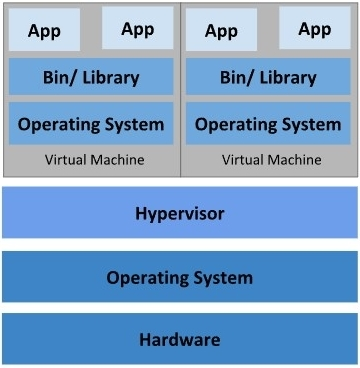
\includegraphics[width=0.6\textwidth]{img/rozdzial1-1.jpg}
    \caption{Wirtualizacja z hipernadzorcą typu drugiego \cite{kubernetes}}
\end{figure}
\newpage

\section{Zastosowania maszyn wirtualnych}
Spośród najpopularniejszych zastosowań maszyn wirtualnych można wyróżnić:
\begin{enumerate}[(1)]
    \item użytkowanie aplikacji lub programów natywnie stworzonych dla konkretnego systemu operacyjnego lub niekompatybilnych z aktualnym systemem,
    \item izolowanie oprogramowania lub wykonywanie zadań potencjalnie niebezpiecznych dla komputera-gospodarza,
    \item testowanie oprogramowania w środowiskach różnych systemów operacyjnych,
    \item przetwarzanie w chmurze \cite{ibm}. 
\end{enumerate}

\section{Zalety i wady wirtualizacji}
Dzięki wirtualizacji możliwe jest efektywne wykorzystywanie zasobów sprzętowych, co przekłada się na niższe koszty eksploatacji hardware'u. Aplikacje w zwirtualizowanym środowisku są odizolowane od siebie i nie mają dostępu do danych przechowywanych na innych wirtualnych maszynach  (Rysunek 1.1), a każda z maszyn ma swój własny system operacyjny, system plików, biblioteki itd. Ponadto aplikacje niekompatybilne z nowszymi wersjami systemu można z powodzeniem uruchamiać w wirtualnych środowiskach. 

Pomimo zmniejszenia ilości sprzętu fizycznego i relatywnie krótkiego czasu, którego potrzebujemy do odtworzenia środowiska, nadal konieczne jest aktualizowanie i utrzymywanie systemów operacyjnych na wirtualnych maszynach. Co więcej, w przypadku problemów sprzętowych dostęp do wszystkich maszyn wirtualnych na danym hoście może być niemożliwy. System operacyjny zajmuje również część pamięci wydzielonej dla konkretnej wirtualnej maszyny, więc jeśli systemy operacyjne dublują się, powstaje problem redundancji, tj. znaczna część miejsca zajmowana jest przez te same systemy \cite{ibm}. 
\newpage

\section{Wykorzystane technologie}
Poniżej krótkie omówienie wykorzystywanych w pracy technologii z otwartym źródłem, umożliwiających wirtualizację w systemach operacyjnych opartych na jądrze Linuxa:
\begin{itemize}
    \item KVM (ang. \textit{Kernel-based Virtual Machine}) \cite{kvm} jest środowiskiem wirtualizacyjnym, wbudowanym bezpośrednio w jądro Linuxa. Funkcję hipernadzorcy pełni samo jądro, a uruchamiane maszyny wirtualne są zwykłymi procesami. 
    
    \item QEMU (\textit{Quick Emulator}) \cite{qemu} to emulator maszyn, który wykorzystywany jest również w roli hipernadzorcy typu drugiego. QEMU zintegrowany z KVM oferuje emulację sprzętową, pozwalając równocześnie na wykonywanie zadań maszyny wirtualnej bezpośrednio na procesorze komputera-gospodarza, osiągając szybkość zbliżoną do maszyn fizycznych. 

    \item Biblioteka \textit{libvirt} \cite{libvirt} składa się z API (ang. \textit{application programming interface}), daemona oraz narzędzi wiersza poleceń. Głównym celem biblioteki jest uproszczenie i ujednolicenie procesu zarządzania maszynami wirtualnymi z różnymi hipernadzorcami. Dzięki wspomnianej bibliotece ułatwiona jest konfiguracja maszyn bazujących na wirtualizacji KVM/QEMU.

    \item Vagrant \cite{vagrant} to otwartoźródłowe oprogramowanie służące do szybkiego tworzenia i konfigurowania maszyn wirtualnych. Do działania niezbędny jest hipernadzorca - najszerzej wspierany przez oprogramowanie jest VirtualBox, jednak udostępniane są również rozszerzenia dla innych platform, w tym \textit{libvirt}. Definiowanie parametrów i budowanie maszyn oparte jest na pliku konfiguracyjnym \textit{Vagrantfile}, w którym umieszczane są informacje o środowisku. Podawany jest konkretny system operacyjny, pakiety i biblioteki do zainstalowania, konfiguracja sieci itp. Dzięki wykorzystaniu plików maszyna o tych samych parametrach może być wielokrotnie tworzona w prosty sposób od nowa. Ponadto Vagrant umożliwia automatyzację, m.in. za pomocą skryptów powłoki czy też Ansible.
\end{itemize}



%%%%%%%%%%%%%%%%%%%%%%%%%%%%%%%%%%%%%%%%%%


\chapter{Konteneryzacja}

Konteneryzacja jest procesem polegającym na spakowaniu aplikacji wraz z niezbędnymi bibliotekami oraz innymi zależnościami do tzw. kontenera (ang. \textit{container}) \cite{biblia_linux}. Kontenery budowane są na podstawie obrazów (ang. \textit{image}) - plików tekstowych, w których definiowana jest pełna konfiguracja.

Kontenery są bardzo lekkie i przenośne, ponieważ nie zawierają pełnego systemu operacyjnego, lecz korzystają z funkcji systemowych komputera-gospodarza (Rysunek 2.1). 

\begin{figure}[h]
    \centering
    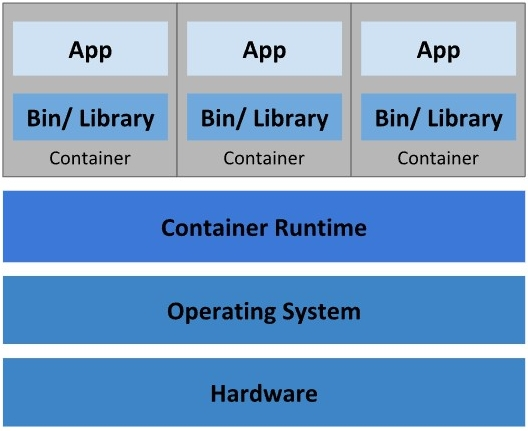
\includegraphics[width=0.6\textwidth]{img/rozdzial1-2.jpg}
    \caption{Konteneryzacja \cite{kubernetes}}
\end{figure}

Pierwszym rozwiązaniem, przypominającym w założeniu współczesne kontenery, była wprowadzona w 2000 roku komenda systemu FreeBSD 4.X \textit{jail} \cite{freebsd, nickoloff}. Umożliwiała ona izolowanie m.in. procesów, sieci, użytkowników i systemów plików. Polecenie miało jednak ograniczenia w zakresie bezpieczeństwa. 

Pięć lat później Google rozpoczęło pracę nad \textit{cgroups}. Mechanizm ten pozwalał nie tylko izolować procesy, ale też ograniczyć zużycie zasobów i wkrótce stał się integralną częścią jądra Linuxa \cite{nickoloff}. 
Od tego momentu rozwijany był również projekt Linux Containers (skrótowo LXC) \cite{lxc}, który miał na celu tworzenie skonteneryzowanych instancji pełnoprawnych systemów linuxowych pozbawionych własnego jądra, a działających bezpośrednio na jądrze systemu-gospodarza. Dzięki temu wewnątrz kontenerów LXC może działać równolegle wiele procesów.

W 2013 roku upublicznione zostało oprogramowanie Docker o otwartym źródle \cite{docker}. Docker, choć korzysta m.in. z \textit{cgroups} oraz rozwiązań LXC, powstał z myślą o tworzeniu kontenerów z tylko jedną aplikacją i ograniczonymi funkcjonalnościami systemu. Obecnie pozostaje najczęściej wykorzystywaną technologią tworzenia kontenerów.

\section{Docker}

Platforma Docker posiada rozbudowany zestaw poleceń, dzięki którym możliwe jest szybkie budowanie, modyfikowanie oraz niszczenie kontenerów. Bardziej optymalną metodą jest jednak tworzenie obrazów poprzez plik tekstowy \textit{Dockerfile}. W pliku tym zawierane są komendy oraz instrukcje dotyczące procesu budowania i konfiguracji. Dzięki temu proces jest zautomatyzowany, a kontener o tej samej specyfikacji może być utworzony ponownie. 

Docker posiada również zestaw dodatkowych funkcjonalności, ułatwiających przechowywanie danych czy też pracę nad złożonymi aplikacjami zbudowanymi z wielu kontenerów. 

Ponadto Docker współtworzy publiczne repozytorium Docker Hub \cite{dockerhub}, gdzie użytkownicy oraz firmy mogą udostępniać stworzone przez siebie obrazy. Tego typu predefiniowane obrazy mogą być pobierane i wykorzystywane w celu dalszej modyfikacji.

\section{Kontenery Dockera a wirtualizacja}

Kontenery Dockera nie wykorzystują wirtualizacji sprzętowej \cite{nickoloff}, która jest kluczowa dla działania maszyn wirtualnych. Wewnątrz znajduje się tylko aplikacja, niezbędne biblioteki oraz ograniczone funkcjonalności systemowe. Uruchomione w kontenerze programy komunikują się bezpośrednio z jądrem systemowym komputera-gospodarza. Brak pełnego systemu operacyjnego sprawia, że kontenery uruchamiane są znacznie szybciej od maszyn wirtualnych \cite{krochmalski}.
 
Kontenery nie są związane z leżącymi poniżej warstwami infrastruktury ani nie są zarządzane przez hipernadzorcę, więc mogą być w niezwykle prosty sposób przenoszone pomiędzy różnymi maszynami lub dostarczycielami rozwiązań chmurowych \cite{poulton}. Umożliwia to przyspieszenie procesu udostępniania, budowania i wdrażania kolejnych wersji oprogramowania.

Nie oznacza to jednak, że wybór jednej z tych technologii ogranicza możliwość użycia drugiej. Obecnie najczęściej spotykane są rozwiązania łączące zarówno wirtualizację, jak i konteneryzację \cite{nickoloff}.

\section{Korzyści i ograniczenia Dockera}

Spośród zalet Dockera można wymienić:

\begin{enumerate}[(1)]
    \item szybkość w tworzeniu, niszczeniu i modyfikowaniu kontenerów,
    \item przenośność, która pozwala na uruchamianie aplikacji na różnych maszynach, 
    \item raz stworzony kontener działa wszędzie tak samo i nie wymaga instalowania dodatkowych paczek po stronie \textit{hosta} - brak konflików związanych z instalacją różnych wersji bibliotek itd.,
    \item niezmienność obrazów - plik \textit{Dockerfile} zapewnia instrukcję instalacyjną do tworzenia kolejnych instancji, 
    \item izolacja aplikacji od siebie, jak i od systemu operacyjnego \cite{nickoloff, krochmalski}.
\end{enumerate}

Należy jednak brać pod uwagę również ograniczenia tej technologii, przede wszystkim:

\begin{enumerate}[(1)]
    \item kontenery, choć szybsze od VM, nie dorównują w szybkości aplikacjom uruchomionym na serwerach fizycznych,
    \item dane zapisywane wewnątrz kontenerów przestają być dostępne wraz z końcem cyklu życia danego kontenera - w celu ich zabezpieczenia należy podjąć dodatkowe kroki (używając np. Docker Volumes),
    \item skonteneryzowanie aplikacji z graficznym interfejsem użytkownika oraz aplikacji monolitycznych jest trudniejsze do wdrożenia i zwykle nieopłacalne - Docker związany jest głównie z mikroserwisami,
    \item w przypadku serwerów środowiska produkcyjnego konieczny jest monitoring i orkiestrator w celu osiągnięcia szybkiej reakcji w przypadku np. awarii serwisów.
\end{enumerate}


%%%%%%%%%%%%%%%%%%%%%%%%%%%%%%%%%%%%%%%%%%


\chapter{Orkiestracja}

Orkiestracja to zautomatyzowany proces konfiguracji, organizacji i kompleksowego zarządzania rozbudowanymi systemami komputerowymi, aplikacjami lub usługami \cite{arundel}. Głównym celem orkiestracji jest zoptymalizowanie działania infrastruktury i zredukowanie do minimum manualnej ingerencji w przypadku powtarzalnych zadań. Stąd głównym zadaniem orkiestratora, czyli narzędzia służącego do orkiestracji, jest utrzymanie systemu w określonym przez administratora stanie.  

Wraz z rozbudową infrastruktury i coraz większą popularnością technologii kontenerowych pojawiła się potrzeba stworzenia zestawu narzędzi, który pozwalał nie tylko na sprawną konfigurację, ale również uruchamianie wielu instancji kontenerów na rozproszonych maszynach. Problem ten próbowała rozwiązać firma Google, która jako jedna z pierwszych wykorzystywała na masową skalę kontenery dla swoich serwisów. Początkowo firma stworzyła własne wewnętrzne oprogramowanie o nazwie Borg, by w 2014 roku udostępnić otwartoźródłowy Kubernetes \cite{kubernetes}.

\section{Kubernetes} 

Kubernetes jest oprogramowaniem służącym do zarządzania kontenerami, planowania i automatyzacji zadań związanych z wdrażaniem oraz skalowaniem skonteneryzowanych aplikacji. Narzędzie dostarcza środowisko dla systemów rozproszonych, w którym działanie kontenerów jest ściśle kontrolowane, a wszelkie zmiany mogą być wdrażane bez przerw w dostępności serwisów. 
\newpage

\section{Składniki Kubernetesa}

Podstawowym, a zarazem najmniejszym obiektem do uruchomienia w Kubernetes jest \textit{pod}. Obiekt ten złożony jest z jednego lub wielu kontenerów działających na tym samym komputerze. 

Obiekty te definiowane są za pomocą plików YAML (\textit{YAML Ain’t Markup Language} - uniwersalny standard serializacji danych \cite{yaml}) i opisują stan oczekiwany klastra. Za ich pomocą możliwe jest określenie m.in. skonteneryzowanych aplikacji na wybranych maszynach, dostępnych dla nich zasobów itd.  

Kontenery powinny być uruchamiane razem w jednym podzie, jeśli są ze sobą świśle związane i muszą współdzielić zasoby takie jak np. dysk \cite{kubernetes}. Ponadto pody mają wspólny adres IP (ang. \textit{Internet Protocol address}) i rozmieszczane są w tzw. węzłach (Rysunek 3.1). 

\begin{figure}[H]
    \centering
    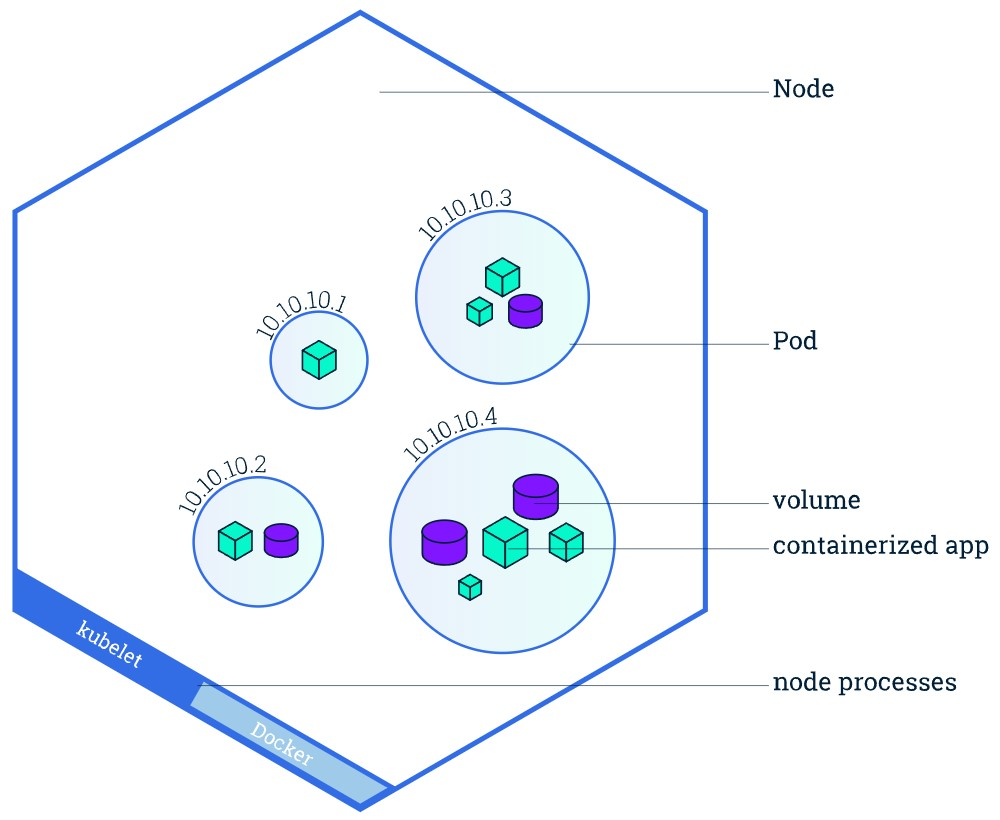
\includegraphics[width=0.6\textwidth]{img/rozdzial1-4.jpg}
    \caption{Przykładowy węzeł z czterema podami - każdy pod posiada własny adres IP dostępny wewnątrz klastra \cite{kubernetes}}
\end{figure}

Klaster (ang. \textit{cluster}) to zbiór maszyn (nazywanych węzłami, ang. \textit{nodes}), na których uruchamiane są skonteneryzowane aplikacje. Węzeł może być maszyną fizyczną lub wirtualną. Każdy klaster musi składać się z przynajmniej jednego węzła, lecz w środowisku produkcyjnym zwykle jest złożony z większej ich liczby. 

Rysunek 3.2 przedstawia przykładowy klaster działający w chmurze - jest zbudowany z trzech węzłów roboczych (ang. \textit{worker nodes}), które zarządzane są przez jeden węzeł warstwy sterowania (ang. \textit{master node}). W takiej konfiguracji węzły robocze odpowiedzialne są za uruchamianie i podtrzymywanie wdrożonych na nich aplikacji, natomiast master monitoruje stan klastra, odpowiada na jego zmieniające się parametry i komunikuje z API dostarczyciela chmury obliczeniowej. 

\begin{figure}[H]
    \centering
    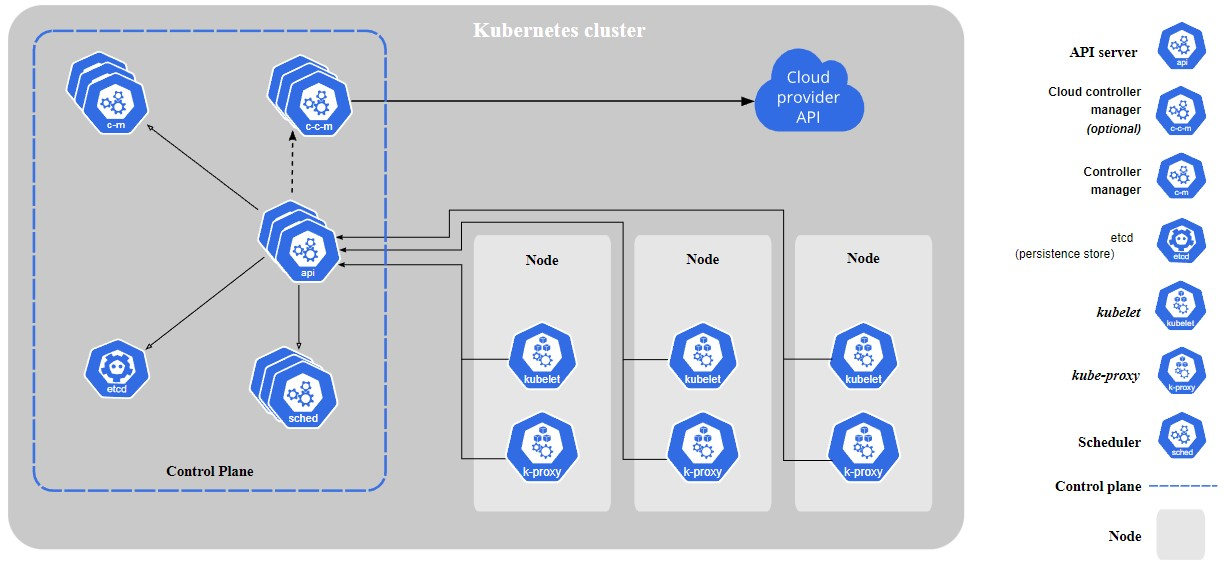
\includegraphics[width=1\textwidth]{img/rozdzial1-3.jpg}
    \caption{Części składowe przykładowego klastra Kubernetes \cite{kubernetes}}
\end{figure}

Składniki Kubernetesa uruchamiane są na każdym węźle, utrzymują działanie podów i definiują środowisko. Składowymi każdego węzła są:
\begin{itemize}
    \item kubelet - odpowiada za uruchamianie kontenerów wewnątrz poda,
    \item kube-proxy - utrzymuje reguły sieciowe węzłów, umożliwiając komunikację między podami a sieciami wewnętrznymi klastra, jak i sieciami zewnętrznymi,
    \item container runtime - oprogramowanie służące do uruchamiania kontenerów, zapewnia obsługę m.in. silnika Dockera.
\end{itemize}

Warstwa sterowania (ang. \textit{control plane}) zarządza klastrem i należącymi do niej podami. Warstwa sterowania może obsługiwać wiele rozproszonych maszyn, zapewniając niezawodność infrastruktury. 

Komponenty warstwy sterowania w wielowęzłowym klastrze zwykle uruchamiane są na osobnej maszynie, gdzie kontenery nie są uruchamiane.\\

Części składowe warstwy sterowania odpowiadają za podejmowanie decyzji oraz wykrywanie zdarzeń w klastrze. Wymienić można poniższe komponenty:

\begin{itemize}
    \item kube-apiserver - główny składnik, udostępnia API, dzięki któremu możliwa jest modyfikacja obiektów i komunikacja między nimi,
    \item etcd - przechowuje dane o klastrze, jego konfigurację i statusy usług,
    \item kube-scheduler - monitoruje tworzenie podów i przypisuje im odpowiednie węzły,
    \item kube-controller-manager - odpowiada za działanie kontrolerów - procesów, które nadzorują stan klastra i w razie potrzeby przywracają klaster do stanu oczekiwanego,
    \item cloud-controller-manager - umożliwia opcjonalne połączenie klastra z usługą chmurową.
\end{itemize}


\section{Funkcjonalności}

Spośród najważniejszych funkcjonalności Kubernetesa można wymienić:
\begin{itemize}
    \item utrzymywanie określonej liczby kontenerów na hoście zgodnej ze stanem oczekiwanym,
    \item możliwość zautomatyzowania procesu tworzenia nowych kontenerów przy wprowadzaniu zmian i zastępowania ich bez utraty dostępności,
    \item balansowanie ruchu (ang. \textit{load balancing}) w celu zapewnienia stabilności infrastruktury,
    \item wykrywanie nowych usług i udostępnianie kontenerów przy pomocy adresu IP lub DNS (ang. \textit{Domain Name System}),
    \item samonaprawa - restartowanie kontenerów, które przestały działać, badanie ich stanu i wymiana na nowe.
\end{itemize}

Kubernetes udostępnia również zestawy narzędzi służących do debugowania, monitorowania oraz zbierania logów. Jednym z nich jest Dashboard - webowy interfejs ogólnego zastosowania, w którym można uzyskać m.in. informacje o stanie klastra i wykorzystywanych zasobach \cite{kubernetes}. Poprzez interfejs możliwe jest również dodawanie nowych obiektów w klastrze oraz edycja już istniejących.
\newpage 

Rysunek 3.3 przedstawia zakładkę podów w interfejsie Dashboardu. Wyświetlona jest lista działających w klastrze podów z informacją o czasie ich działania, statusie oraz indywidualnym zużyciu pamięci oraz procesora. Powyżej listy znajdują się takżę dwa wykresy obrazujące skumulowane wykorzystanie zasobów przez pody. 
\vspace{2em}

\begin{figure}[h]
    \centering
    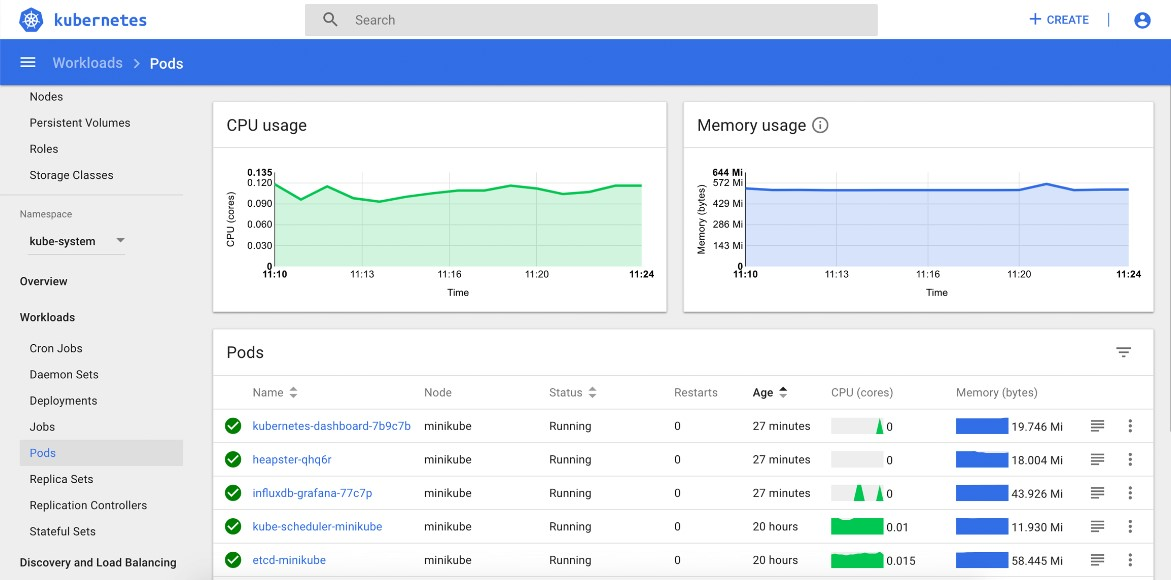
\includegraphics[width=1\textwidth]{img/rozdzial1-52.jpg}
    \caption{Kubernetes Dashboard - interfejs \cite{kubernetes}}
\end{figure}

%%%%%%%%%%%%%%%%%%%%%%%%%%%%%%%%%%%%%%%%%%


\chapter{Dodatkowe narzędzia}

Przy tworzeniu projektu wykorzystano również narzędzia open source, umożliwiające testowanie i monitorowanie klastra czy też zautomatyzowanie czynności w infrastrukturze.

\section{Automatyzacja zadań}

\begin{itemize}
    \item Helm \cite{helm} to opracowany dla Kubernetesa menedżer pakietów, który znacznie ułatwia instalację i zarządzanie wstępnie skonfigurowanymi aplikacjami. Pakiety, nazywane \textit{chart}, są tworzone i umieszczane w repozytoriach, by następnie ściągnąć je i uruchomić w środowisku klastra. Gotowe charty publikowane są na stronie internetowej Artifact Hub \cite{artifacthub}.

    %\item Ansible \cite{ansible} jest wieloplatformowym narzędziem służącym do automatyzacji zadań związanych z instalacją i konfiguracją systemów operacyjnych. W plikach YAML, zwanych \textit{playbookami}, opisywany jest stan oczekiwany systemu. Ansible umożliwia uruchamianie playbooków na wielu hostach.
\end{itemize}

\section{Monitoring}

Jako dopełnienie funkcjonalności interfejsu Kubernetes Dashboard wykorzystano poniższe platformy:

\begin{itemize}
    \item Prometheus \cite{prometheus} to zbiór aplikacji służących do zbierania i przechowywania danych szeregu czasowego oraz przesyłania alertów. Wykorzystanie bazy danych szeregów czasowych (ang. \textit{time series database}) pozwala na analizę danych w porządku czasowym i przedstawienie ich w formie wykresu, gdzie na osi X znajdują się przedziały czasu. Ponadto Prometheus oferuje własny język zapytań PromQL.

    \item Grafana \cite{grafana} służy do monitoringu i wizualizacji danych z wybranego źródła - narzędzie obsługuje większość popularnych baz danych różnego rodzaju. Grafana przedstawia zebrane dane w formie wykresów. Możliwe jest importowanie predefiniowanych dashboardów lub tworzenie własnych, co pozwala na dużą personalizację. 
\end{itemize}

\section{Testowanie}

Testy wydajnościowe mają na celu sprawdzenie badanej infrastruktury pod kątem spełnienia określonych wymagań, np. szybkości działania, dostępności itp. 

W projekcie wykorzystano dwa rodzaje testów: obciążeniowe (ang. \textit{load testing}) oraz przeciążające (ang. \textit{stress testing}). Pierwszy z nich sprawdza działanie infrastruktury przy przewidywanym obciążeniu ze strony np. użytkowników i wynikającego z tego ruchu sieciowego. Z kolei drugi wymieniony rodzaj testu polega na doprowadzeniu infrastruktury do skrajnej sytuacji, takiej jak pełne obciążenie CPU (ang. \textit{central processing unit}), pamięci itd.

Do przeprowadzenia testów wykorzystano oprogramowanie:
\begin{itemize}
    \item Narzędzie K6 \cite{k6} służy do tworzenia testów wydajnościowych, m.in. obciążenia serwisów. Skrypty testów tworzone są w języku JavaScript. Oprogramowanie pozwala na tworzenie tzw. wirtualnych użytkowników, symulujących prawdziwy ruch sieciowy. Ponadto przy pisaniu skryptów deklarowany jest czas trwania testu oraz jego fazy, w których ruch może ulec zmianie itp., co pozwala na dostosowanie testów do wymagań i charakteru infrastruktury. 

%    \item KBoom \cite{kboom} to prosty program sprawdzający szybkość i skalowalność klastra, tworząc wybraną ilość podów w interwałach. 
    
    \item Kube-Stresscheck \cite{stress} bazuje na popularnym w systemach linuxowych programie \textit{stress}, który w pętli oblicza pierwiastek kwadratowy losowych liczb. Narzędzie pozwoli sprawdzić jak zachowuje się infrastruktura i klaster pod dużym obciążeniem procesora i pamięci. 
\end{itemize}